\documentclass[11pt,a4paper,twoside,openright,titlepage,
headinclude,footinclude,BCOR5mm,
numbers=noenddot,cleardoublepage=empty,
tablecaptionabove]{scrbook}
\usepackage[T1]{fontenc}
\usepackage[utf8]{inputenc}
\usepackage[italian]{babel}
\usepackage[eulerchapternumbers,beramono,eulermath, pdfspacing]{classicthesis}
\usepackage{arsclassica}
\usepackage{graphicx}
\usepackage{subfig}
\usepackage{caption}
\usepackage{amsmath}
\usepackage{amsthm}
\usepackage{color}
\usepackage{listings}
\usepackage{xcolor}
\makeindex
\definecolor{mio_colore}{RGB}{242,243,244}
\definecolor{dkgreen}{rgb}{0,0.6,0}
\definecolor{gray}{rgb}{0.5,0.5,0.5}
\lstset{language=Octave,showstringspaces=false,basicstyle=\small\ttfamily,literate={à}{{\'a}}1 {ã}{{\~a}}1 {è}{{\'e}}1 {ù}{{\'u}}1{l'}{{l'}}2{n'}{{n'}}2{L'}{{L'}}2, backgroundcolor=\color{mio_colore},numberstyle=\tiny\color{gray},
            keywordstyle=\color{blue},commentstyle=\color{dkgreen},stringstyle=\color{red},}
            
            
\begin{document}

La funzione newton\_D1\_vett è:
\begin{lstlisting}[frame=trBL]
function A=newton_D1_vett(x_0,y_0,m,l)
%funzione che costruisce l'immagine di centro x_0+I*y_0
%di semilato l e con (2*m+1)x(2*m+1) punti
I=sqrt(-1);
maxiteration=100;
h=l/m;
Z = (x_0+I*y_0)+(h*ones(2*m+1,1)*[-m:m]-I*h*[-m:m]'*ones(1,2*m+1));
r=roots([1,0,10000,-200,1]);
A=zeros(2*m+1,2*m+1,3);
CONT=zeros(2*m+1);
%calcoliamo la trasformazione di Z con il metodo di Newton
%e salviamo nella matrice CONT il numero di iterazioni necessarie
%a far si che sul pixel (i,j) sia verificata la condizione 
%richiesta
for k = 1:maxiteration
Z = Z-(Z.^4+(100*Z-1).^2)./(4*Z.^3+20000*Z-200);
CONT=CONT+abs(abs(Z-r(1))<1.e-04*abs(r(1)))+...
+abs(abs(Z-r(2))<1.e-04*abs(r(2)))+...
+abs(abs(Z-r(3))<1.e-04*abs(r(3)))+...
+abs(abs(Z-r(4))<1.e-04*abs(r(4)));
end
%dividiamo punto a punto i pixel dell'immagine per il relativo 
%valore in CONT
CONT=(maxiteration+1)*ones(2*m+1)-CONT;
A(:,:,1) = (abs(abs(Z-r(1)) < 1.e-4*abs(r(1)))+...
+abs(abs(Z-r(4)) < 1.e-4*abs(r(4))))./CONT;
A(:,:,2) = (abs(abs(Z-r(2)) < 1.e-4*abs(r(2)))+...
+abs(abs(Z-r(4)) < 1.e-4*abs(r(4))))./CONT;
A(:,:,3) = (abs(abs(Z-r(3)) < 1.e-4*abs(r(3))))./CONT;
%normalizziamo gli elementi della matrice, in modo da
%assegnare al punto di valore maggiore la luminosità massima
A=A./max(max(max(A)));
%decommentare per stampare l'immagine automaticamente
%imshow(A);
endfunction
\end{lstlisting}

Dando i comandi:
\begin{lstlisting}[frame=lines]
>>A=newton_D1_vett(0,0,200,5*10^6);
>>imwrite(A,'semilato_5*10^6.jpg')
>>A=newton_D1_vett(1/100,0,200,10^-3);
>>imwrite(A,'semilato_10^-3.jpg')
>>A=newton_D1_vett(1/100,0,200,10^-4);
>>imwrite(A,'semilato_10^-4.jpg')
>>A=newton_D1_vett(1/100,0,200,10^-5);
>>imwrite(A,'semilato_10^-5.jpg')
\end{lstlisting}
otteniamo le immagini richieste:
\begin{figure}[h!]
\centering
\subfloat[][\emph{semilato $5*10^6$}]
    {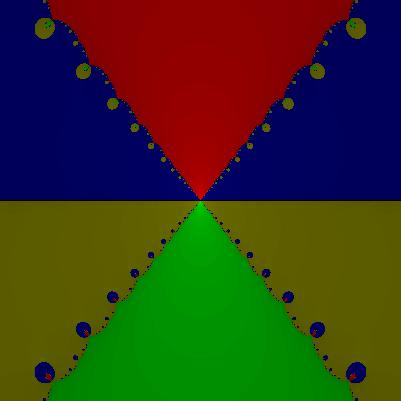
\includegraphics[width=.45\textwidth]{figs/semilato_5*10^6.jpg}} \quad
\subfloat[][\emph{semilato $10^{-3}$}]
    {
\includegraphics[width=.45\textwidth]{figs/semilato_10^-3.jpg}} \\
\subfloat[][\emph{semilato $10^{-4}$}]
    {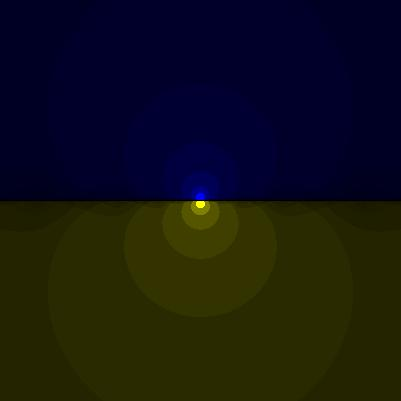
\includegraphics[width=.45\textwidth]{figs/semilato_10^-4.jpg}} \quad
\subfloat[][\emph{semilato $10^{-5}$}]
    {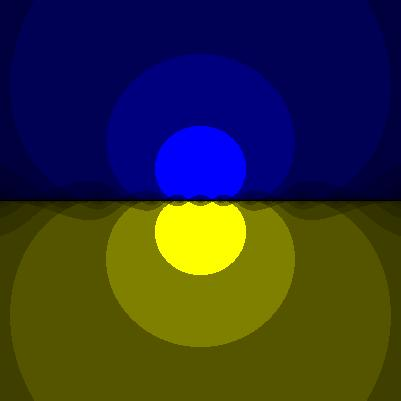
\includegraphics[width=.45\textwidth]{figs/semilato_10^-5.jpg}}
\caption{Frattale con vari centri e semilati.}
\end{figure}
\newpage
La funzione mandelbrot\_E0 è:
\begin{lstlisting}[frame=trBL]
function mandelbrot_E0(p,l,m)
%funzione che disegna il frattale di mandelbrot
%con lato l, centro p e numero di punti
%(2*m+1)x(2*m+1)
I = sqrt(-1);
h=l/m;
A = h*ones(2*m+1,1)*[-m:m]-I*h*[-m:m]'*ones(1,2*m+1)+p;
q=63;
cont=zeros(2*m+1);
Z=zeros(2*m+1);
for i=1:q
Z=Z.^2+A;
cont=cont+i*abs(abs(Z)>2);
Z=Z.*abs(cont==0);
A=A.*abs(cont==0);
end
cont=cont+64*abs(cont==0);
colormap('default');
imshow(cont,colormap);
\end{lstlisting}
Da questa funzione, assegnando i valori $p=-1.5$ e $l=2$, 
$p=\phi-2+i(\phi-1)$ e $l=0.5, 0.1, 0.01$, con $\phi=(1+\sqrt{5})/2$, 
si ottengono le seguenti immagini:
\begin{figure}[h!]
\centering
\subfloat[][\emph{$p=-1.5$, $l=2$}]
    {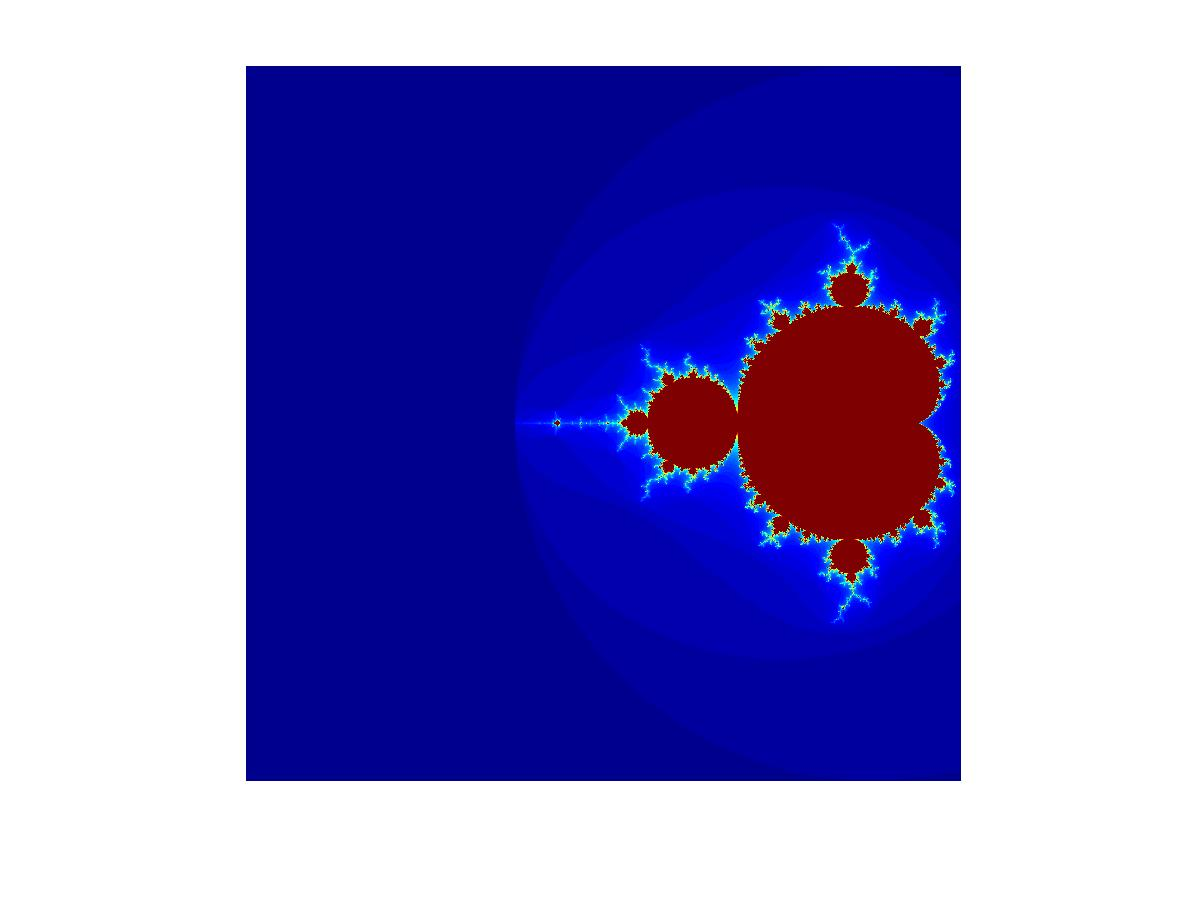
\includegraphics[width=.45\textwidth]{figs/Primo_frattale.jpg}} \quad
\subfloat[][\emph{$p=\phi-2+i(\phi-1)$, $l=0.5$}]
    {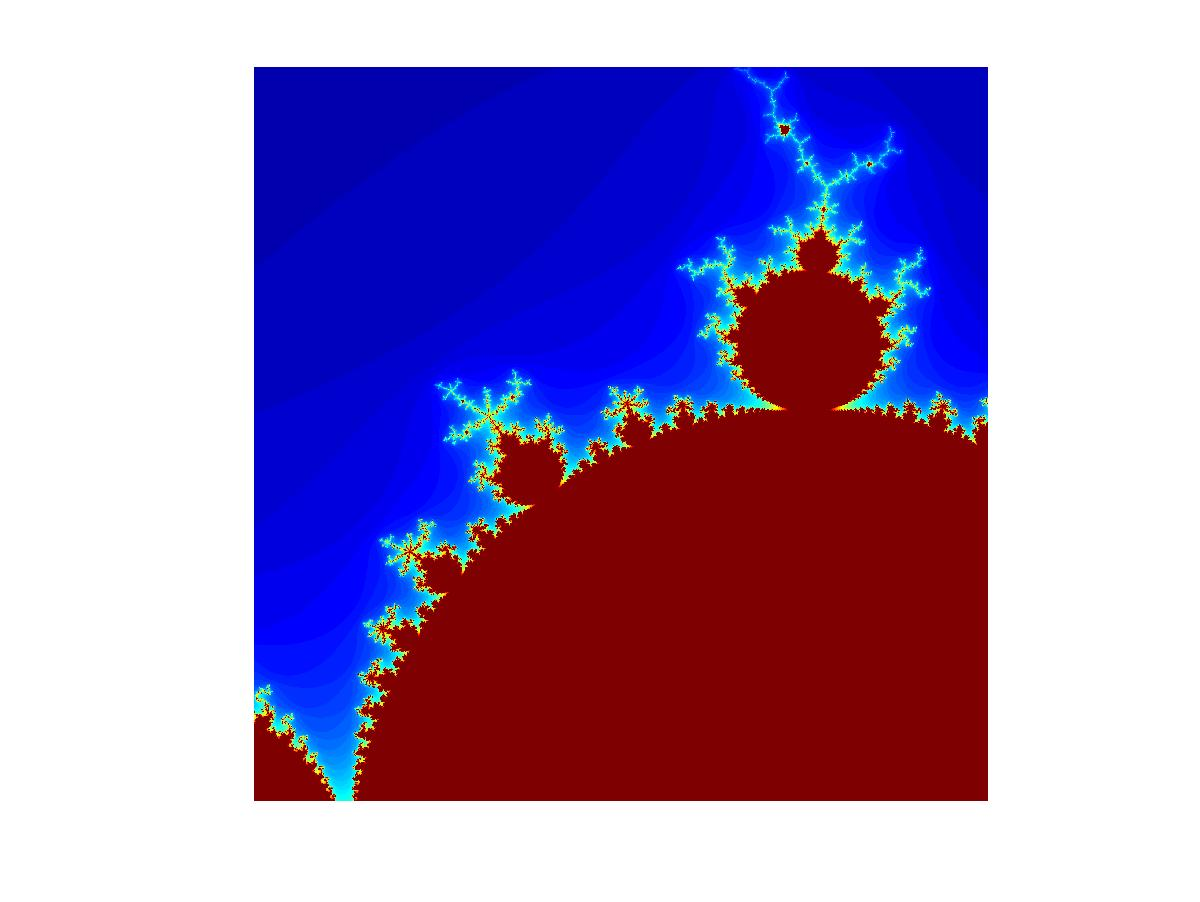
\includegraphics[width=.45\textwidth]{figs/Secondo_frattale.jpg}} \\
\subfloat[][\emph{$p=\phi-2+i(\phi-1)$, $l=0.1$}]
    {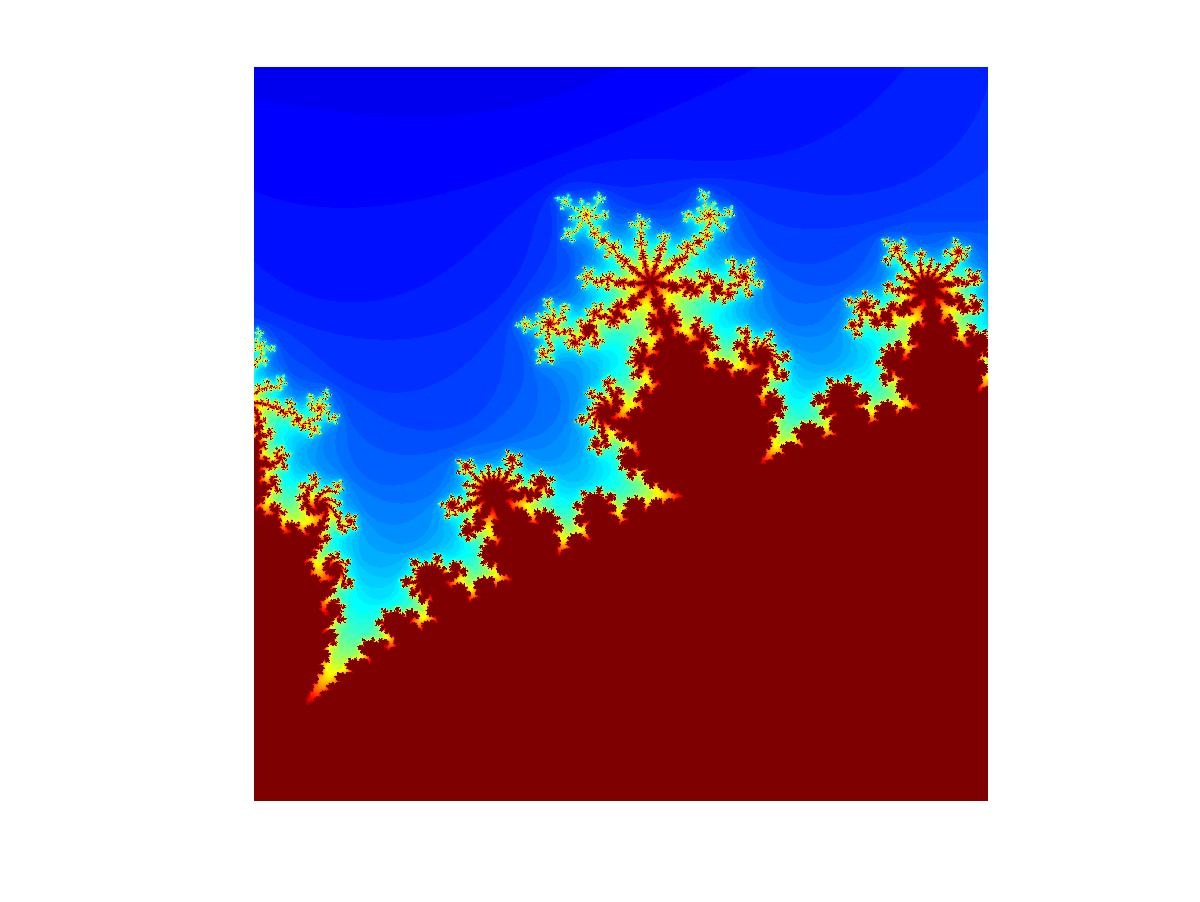
\includegraphics[width=.45\textwidth]{figs/Terzo_frattale.jpg}} \quad
\subfloat[][\emph{$p=\phi-2+i(\phi-1)$, $l=0.01$}]
    {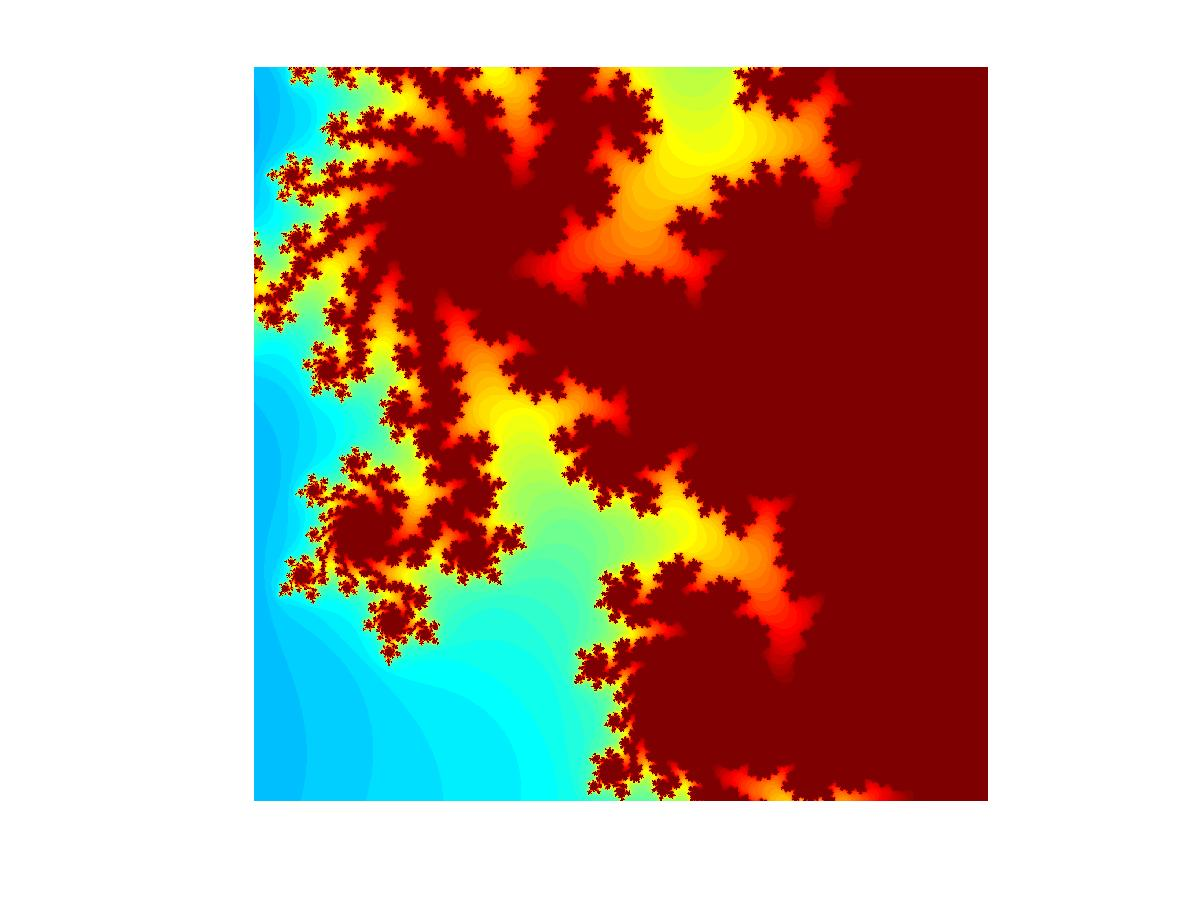
\includegraphics[width=.45\textwidth]{figs/Quarto_frattale.jpg}}
\caption{Frattali di Mandelbrot con diversi valori di centro e semilato.}
\end{figure}

\end{document}
